\subsection{Strømforsyning Design}
\label{ch:stroemforsyning_design}

Strømforsyningen skal levere 12V DC til steppermotoren og de fire ventilatorer og 5V DC til PSoC 4 Pioneer Kits og Mosfetdriver til Varmelegeme.
Et Multisim diagram for designet er vist på Figur \ref{fig:multisim_stroemforsyning}.

\begin{figure}[h]
\centering 
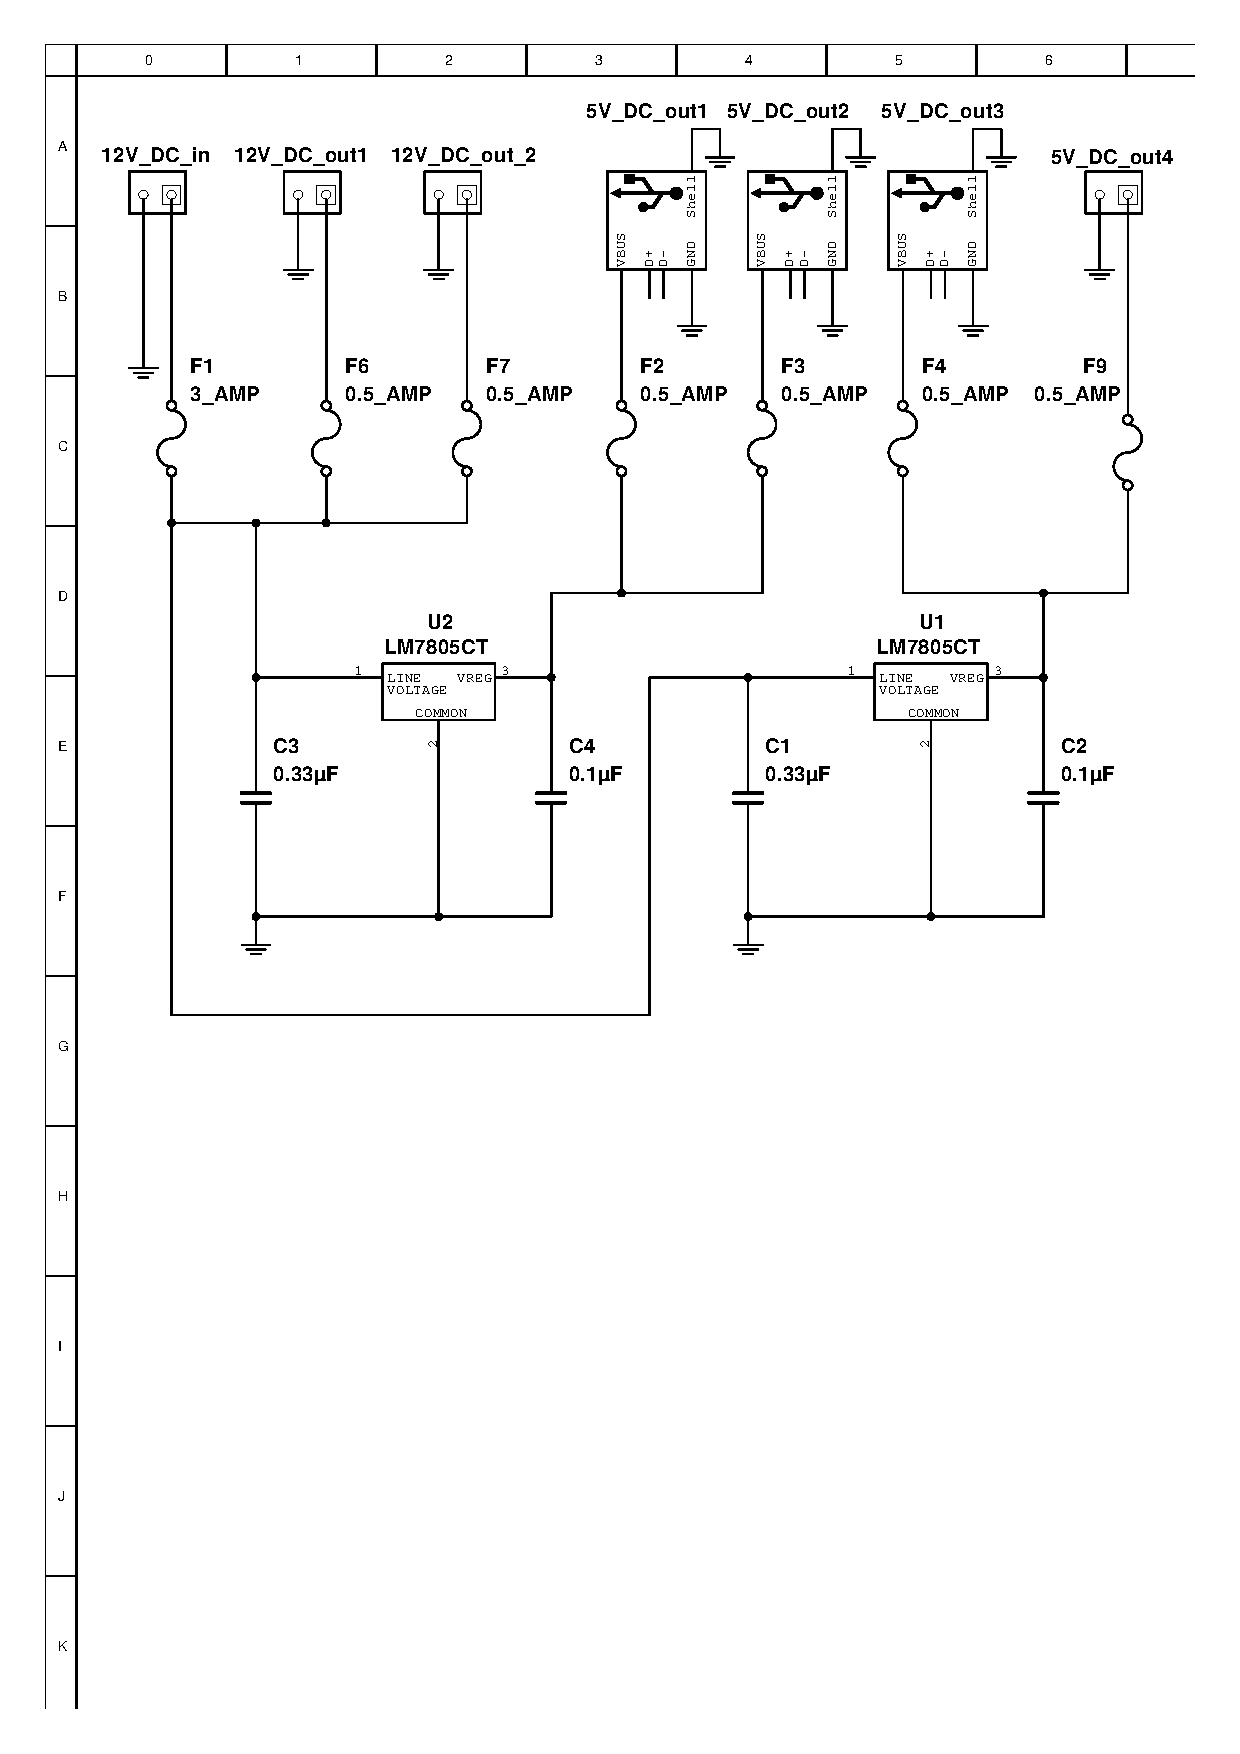
\includegraphics[width={\textwidth}, trim=50 350 30 40, clip=true] {../fig/multisim_stroemforsyning.pdf}
\caption{Diagram for blokken Strømforsyning}
\label{fig:multisim_stroemforsyning}
\end{figure}

Designet er forsynet med sikringer jf. \ref{P-subsec:signalbeskrivelser} \nameref{P-subsec:signalbeskrivelser} på side \pageref{P-subsec:signalbeskrivelser} i projektdokumentationen.
5V DC forsyningerne laves vha. en spændingsregulator - LM7805 - som er anvendt jf. standard applikationen i databladet \cite{lib:LM7805_DS}.
Der kan afsættes op til 7 W i hver af de to spændingsregulatorer, derfor monteres de med køleplade.

\mbox{}

For yderligere info se afsnit \ref{P-sec:Stroemforsyning_Design} \nameref{P-sec:Stroemforsyning_Design} på side \pageref{P-sec:Stroemforsyning_Design} i projektdokumentationen.

\clearpage